\chapter[Experimental Setup]{The CMS experiment}
\label{chap:CMSExp}
%During the Run II, the Large Hadron Collider (LHC) has produced 
%produced proton-proton collisions at an unprecedented ~\centermassenergy, 
%and at a high luminosity never reached before for 
The CMS experiment is the biggest multi-purpose particle detector
ever built in the world and  is located on the Large Hadron Collider, or LHC \cite{chp2:LHCTDR}. The LHC is a proton accelerator placed at the CERN 
laboratory in Switzerland. The unprecedented \centermassenergy~
of the proton-proton collisions produced by this accelerator and its 
very high luminosity reached, make possible the search
for Physics BSM in a higher energy spectrum. The data used for this dissertation comes from
$pp$ collisions produced by the LHC at \sqrts 13 TeV, and recorded by the CMS experiment during 2016.
In the present Chapter, the LHC accelerator and the CMS experiment will be
described making emphasis on the CMS subdetectors involved with the 
tau-lepton detection, which plays an important role in this work. 

%This Chapter is organized as follows: First, a brief description of the LHC accelerator is presented;
%next, the CMS subdetector and its subdetectors are described; and finally, the chapter finishes with a brief 
%description of physic objects reconstructed by CMS

\section{LHC Accelerator}
\label{sec:LHC}
The LHC is a particle accelerator designed to collide protons (or lead ions) at a \centermassenergy~up to 14 TeV. The 
LHC accelerates protons along two rings of 27 km of circumference, installed in a tunnel 
approximately 100 m underground of the French-Swiss border. Bunches of protons (or ions)
are accelerated, using ratio frequency (RF) cavities, along the rings in opposite directions and they collide in 
different points where dedicated experiments are placed in order to detect the products of the collisions. The four experiments
are: CMS \cite{chp2:CMSTDR,chp2:CMSTDR2}, ATLAS \cite{chp2:ATLASTDR}, LHCb \cite{chp2:LHCb} and  ALICE \cite{chp2:ALICETDR} (See Figure \ref{chp2:LHCringsfigure}). CMS 
and ATLAS are multi-purpose detectors optimized for the discovery of new physics BSM. The aim of the LHCb detector is to study 
the charge-parity (CP) symmetry violation, which is been postulated to explain the unknown matter-antimatter 
asymmetry. The ALICE detector is specialized in studying the quark-gluon plasma, state in 
which the quarks behave asymptotically as free particles. Besides, there are two additional smaller 
experiments: TOTEM and LHCf. TOTEM searches for accurate measurements of total, elastic and diffractive
cross sections. The LHCf purpose is to study the high energy cosmic rays regime by using the particles thrown forward by collisions.

\begin{figure}[ht]
\begin{center}
 \scalebox{0.35}{
          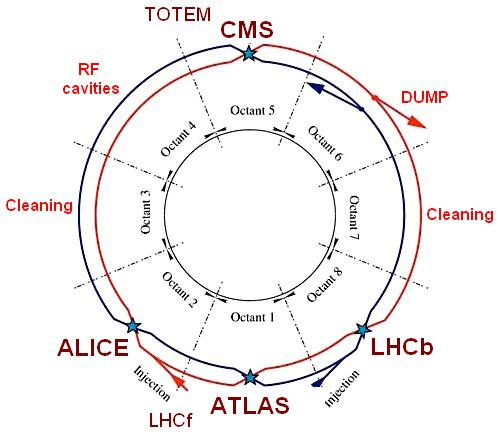
\includegraphics{figuras/Chapter2/LHCrings}}
\caption{Schematic view of the LHC proton rings with the interaction points, 
where the CMS, ATLAS, ALICE and LHCb detectors are located.}\label{chp2:LHCringsfigure}
\end{center}
\end{figure}

\subsection{LHC Pronton Accelerator Chain}
\label{subsec:ProtonAcceleratorChain}

%at an energy of 450 GeV, they have several

Before protons are injected into the two LHC rings (also known as LHC main ring), they have several
pre-acceleration stages  shown in Figure \ref{chp2:LHCaccelerationchain}. The process starts with the extraction of protons 
in the Duoplasmatron Proton Ion Source. In the proton source, the protons are 
extracted by ionization of Hydrogen gas in so called ``\textit{bunches}''; bunches of protons 
afterwards will be accelerated together in order to increase their probability to collide. As 
result, bunches of protons are injected into a linear accelerator, Linac2, where their energy is increased up to 50 MeV. Once the protons 
reach such energy, they are delivered to the Proton Synchrotron Booster (PSB) and then to the
Proton Synchrotron (PS) where they are accelerated up to 1.4 GeV and 25 GeV, respectively. Additionally,
in the PS the bunches of protons are splitted into bunches spaced by 
25 ns\footnote{The spacing between bunches is generally known as \textit{Bunch Crossing}. For the Run I, the bunches were spaced by 50 ns}. Finally, 
the pre-acceleration chain finishes in the Super Proton Synchrotron (SPS), where 
the protons reach an energy up to 450 GeV before they are injected into the LHC rings. 

\begin{figure}[ht]
\begin{center}
 \scalebox{0.3}{
          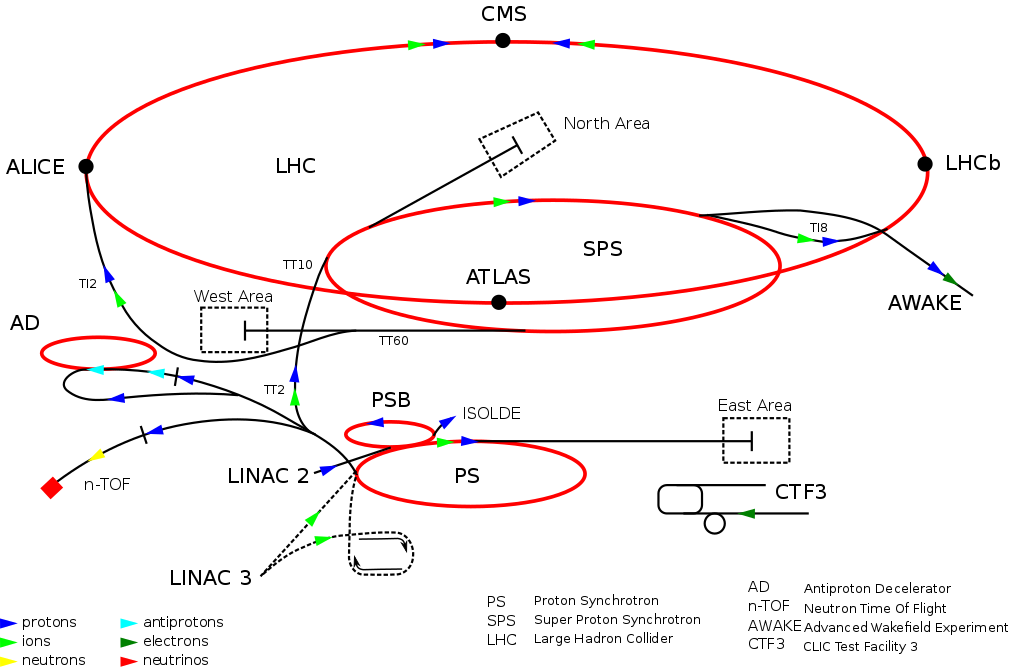
\includegraphics{figuras/Chapter2/LHCaccelerationchain2}}
\caption{Schematic view of the proton accelerator chain at CERN.}\label{chp2:LHCaccelerationchain}
\end{center}
\end{figure}

The bunches of protons are injected into the LHC rings in opposite directions, clockwise and 
counter-clockwise, where they can reach an energy up to 7 TeV and finally could collide at a maximum of
\centermassenergy~of 14 TeV in the interaction points. The protons are accelerated inside the two 
beam pipes using 8 RF cavities. The RF cavities operate to a frequency of 400 MHz in the final 
stage and the gradient of the electric field produced is 5 MV/m approximately. The RF cavities also
ensures the longitudinal stability of the beams. The LHC uses 1232 superconductor dipole magnets, where 
each one produces a magnetic field strength up to 8.3 T, for bending the beam along the rings. The dipoles 
are cooled by superfluid helium at a temperature of 1.9 K, that also helps to optimize the vacuum
inside the beam pipe. The bunches of protons are radially focused by 392 quadrupole magnets placed
along the LHC rings, each 5-7 m long. The radial focusing is important as well to increase 
the collision probability since the protons within a bunch will be placed in a smaller cross-section. \\

\subsection{Luminosity}
\label{sec:Luminosity}


\subsection{Runs at the LHC}
\label{sec:LHCRuns}

\section{The CMS Detector}
\label{sec:CMS}

\section{The Tracker System}
\label{sec:Tracker}

\subsection{Pixel Tracker}
\label{subsec:Pixel}

\subsection{Silicon Strip Detector}
\label{subsec:Strip}

\section{Electromagnetic Calorimeter}
\label{sec:ECal}

\section{Hadronic Calorimeter}
\label{sec:HCal}

\section{Muon System}
\label{sec:MuonSys}

\subsection{RPCs}
\label{subsec:RPCs}

\subsection{DTs}
\label{subsec:DTs}

\subsection{CSCs}
\label{subsec:CSCs}

\subsection{GEMs}
\label{subsec:GEMs}

\section{Particle Reconstruction}
\label{sec:ParticleReconstruction}

\subsection{Trigger}
\label{subsec:Trigger}

\subsection{Data Adquisition}
\label{subsec:DAQ}

\subsection{Physics Objects}
\label{subsec:PhysicsObjects}
